\documentclass[11pt]{article}
\usepackage[margin=1in]{geometry}
\usepackage{amsmath,amssymb,amsthm}
\usepackage{graphicx}
\usepackage{microtype}
\usepackage[colorlinks=true,linkcolor=blue,citecolor=blue,urlcolor=blue]{hyperref}

\newtheorem{theorem}{Theorem}
\newtheorem{lemma}{Lemma}
\newcommand{\R}{\mathbb R}
\newcommand{\dom}{\operatorname{dom}}

\title{Boundedness cannot be dropped in Theorem 3.5\\of arXiv:2112.13900}
\author{Candidate counterexample packet}
\date{12 August 2026}

\begin{document}
\maketitle

\noindent\fbox{\parbox{0.94\textwidth}{
\textbf{Status: candidate full counterexample, likely valid.}
The literal open problem has a negative answer, already in the one-dimensional Hilbert space.  The example is not quasibounded, so the stronger replacement question proposed in the next sentence of the source remains open.
}}

\section{Source problem}

Adhikari--Aryal--Bhatt--Kunwar--Puri--Ranabhat prove the following annular existence theorem for a bounded, maximal monotone, positively homogeneous operator $A$; its boundary assumptions are denoted (H3) and (H4) in the source \cite{source}.

\begin{figure}[ht]
\centering
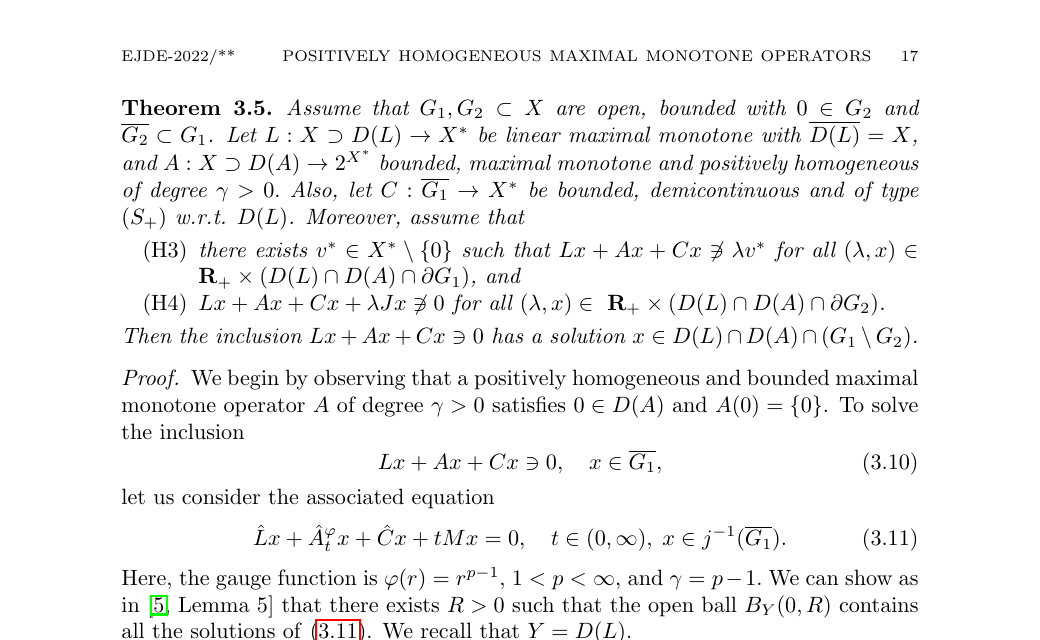
\includegraphics[width=0.96\textwidth]{figures/theorem_3_5_crop.png}
\caption{Theorem 3.5 in the source PDF, page 17.}
\end{figure}

They then ask whether boundedness of $A$ can be dropped, and suggest quasiboundedness as a possible replacement.

\begin{figure}[ht]
\centering

\includegraphics[width=0.96\textwidth]{figures/open_problem_crop.png}
\caption{Open Problem 3.1 in the source PDF, page 20.}
\end{figure}

\section{Counterexample}

\begin{theorem}
The conclusion of Theorem 3.5 is false if the boundedness assumption on $A$ is simply deleted.  This holds for every prescribed degree $\gamma>0$.
\end{theorem}

\begin{proof}
Work in the real Hilbert space $X=\R$, identified with its dual.  Fix $\gamma>0$ and define the proper lower-semicontinuous convex function
\[
 \Phi(x)=
 \begin{cases}
   \dfrac{x^{\gamma+1}}{\gamma+1},&x\geq0,\\[4pt]
   +\infty,&x<0.
 \end{cases}
\]
Let $A=\partial\Phi$.  Explicitly,
\begin{equation}\label{Adef}
 \dom A=[0,\infty),\qquad
 A(0)=(-\infty,0],\qquad
 A(x)=\{x^\gamma\}\quad(x>0).
\end{equation}
Because $A$ is the subdifferential of a proper lower-semicontinuous convex function, it is maximal monotone.  Formula \eqref{Adef} also verifies the source definition of positive homogeneity: for $s>0$, $A(sx)=s^\gamma A(x)$, including $x=0$ since every positive dilation preserves the negative ray; for $s=0$, the required inclusion $0^\gamma A(x)\subset A(0)$ holds.  The operator is not bounded in the source's sense, because the bounded set $\{0\}$ has the unbounded image $A(0)$.

Now take
\[
 L=0,\qquad C=0,\qquad G_1=(-2,2),\qquad G_2=(-1,1),
 \qquad v^*=-1.
\]
The zero operator $L$ is linear maximal monotone with full domain.  The map $C$ is bounded and demicontinuous.  It is of type $(S_+)$ with respect to $\dom L$ because weak and norm convergence coincide in $\R$.  The sets are open and bounded, $0\in G_2$, and $\overline{G_2}\subset G_1$.

It remains to check the two boundary hypotheses.  Since
\[
 \dom A\cap\partial G_1=\{2\},
\]
we have
\[
 L2+A2+C2=\{2^\gamma\},
 \qquad \lambda v^*=-\lambda\leq0\quad(\lambda\geq0).
\]
Thus (H3) holds.  Similarly, $\dom A\cap\partial G_2=\{1\}$ and the normalized duality map on $\R$ is $Jx=x$, so
\[
 L1+A1+C1+\lambda J1=\{1+\lambda\}\not\ni0
 \qquad(\lambda\geq0).
\]
Hence (H4) holds.

Finally,
\[
 0\in Lx+Ax+Cx=Ax
 \quad\Longleftrightarrow\quad x=0.
\]
Indeed $0\in A(0)$, while $A(x)=\{x^\gamma\}>0$ for $x>0$ and $A$ is undefined for $x<0$.  But $0\in G_2$, so $0\notin G_1\setminus G_2$.  There is therefore no solution in
$\dom L\cap\dom A\cap(G_1\setminus G_2)$, contrary to the conclusion of Theorem 3.5.
\end{proof}

\section{Why this does not settle the quasibounded variant}

The source defines $A$ to be quasibounded when, for every $S>0$, the conditions
\[
 \|x\|\leq S,\qquad \langle x^*,x\rangle\leq S\|x\|,
 \qquad x^*\in Ax
\]
force a uniform bound on $\|x^*\|$.  The operator \eqref{Adef} fails this at $x=0$: every $x^*\leq0$ belongs to $A(0)$ and satisfies the displayed pairing inequality, but $|x^*|$ is unbounded.

This pinpoints the first obstruction.  Positive homogeneity makes $A(0)$ dilation-invariant.  Quasiboundedness at zero would force $A(0)$ to be bounded, hence $A(0)=\{0\}$.  The source proof also uses boundedness to obtain compactness of the Yosida approximants; those later uses are not repaired merely by assuming $A(0)=\{0\}$.  Thus the packet proves exactly the negative answer to the literal first sentence, while making no claim about the stronger quasibounded replacement.

Five focused upgrade attempts are recorded in the accompanying attempt note.  In particular, finite-dimensional quasibounded examples are structurally blocked, and the natural infinite-dimensional linear route collides with (H3).  No later paper or explicit answer to this open problem was found in bounded exact-phrase, title, author, and structural searches through 12 August 2026.

\section{Verification}

The script \texttt{code/verify\_counterexample.py} checks exact rational samples of monotonicity, the two boundary conditions, and absence of annular zeros.  It reports
\begin{quote}\ttfamily
PASS: monotonicity samples, (H3), (H4), and absence of annular zeros.
\end{quote}
The computational check is supplementary; maximal monotonicity follows analytically from the subdifferential representation.

\begin{thebibliography}{1}
\bibitem{source}
D. R. Adhikari, A. Aryal, G. Bhatt, I. J. Kunwar, R. Puri, and M. Ranabhat,
\emph{Solvability of inclusions involving perturbations of positively homogeneous maximal monotone operators},
Electronic Journal of Differential Equations 2022, no. 63, 1--25;
\href{https://arxiv.org/abs/2112.13900}{arXiv:2112.13900}.
\end{thebibliography}

\end{document}
